\documentclass{article} % For LaTeX2e
\usepackage{iclr2027_conference,times}

% Optional math commands from https://github.com/goodfeli/dlbook_notation.
%%%%% NEW MATH DEFINITIONS %%%%%

\usepackage{amsmath,amsfonts,bm}

% Mark sections of captions for referring to divisions of figures
\newcommand{\figleft}{{\em (Left)}}
\newcommand{\figcenter}{{\em (Center)}}
\newcommand{\figright}{{\em (Right)}}
\newcommand{\figtop}{{\em (Top)}}
\newcommand{\figbottom}{{\em (Bottom)}}
\newcommand{\captiona}{{\em (a)}}
\newcommand{\captionb}{{\em (b)}}
\newcommand{\captionc}{{\em (c)}}
\newcommand{\captiond}{{\em (d)}}

% Highlight a newly defined term
\newcommand{\newterm}[1]{{\bf #1}}


% Figure reference, lower-case.
\def\figref#1{figure~\ref{#1}}
% Figure reference, capital. For start of sentence
\def\Figref#1{Figure~\ref{#1}}
\def\twofigref#1#2{figures \ref{#1} and \ref{#2}}
\def\quadfigref#1#2#3#4{figures \ref{#1}, \ref{#2}, \ref{#3} and \ref{#4}}
% Section reference, lower-case.
\def\secref#1{section~\ref{#1}}
% Section reference, capital.
\def\Secref#1{Section~\ref{#1}}
% Reference to two sections.
\def\twosecrefs#1#2{sections \ref{#1} and \ref{#2}}
% Reference to three sections.
\def\secrefs#1#2#3{sections \ref{#1}, \ref{#2} and \ref{#3}}
% Reference to an equation, lower-case.
\def\eqref#1{equation~\ref{#1}}
% Reference to an equation, upper case
\def\Eqref#1{Equation~\ref{#1}}
% A raw reference to an equation---avoid using if possible
\def\plaineqref#1{\ref{#1}}
% Reference to a chapter, lower-case.
\def\chapref#1{chapter~\ref{#1}}
% Reference to an equation, upper case.
\def\Chapref#1{Chapter~\ref{#1}}
% Reference to a range of chapters
\def\rangechapref#1#2{chapters\ref{#1}--\ref{#2}}
% Reference to an algorithm, lower-case.
\def\algref#1{algorithm~\ref{#1}}
% Reference to an algorithm, upper case.
\def\Algref#1{Algorithm~\ref{#1}}
\def\twoalgref#1#2{algorithms \ref{#1} and \ref{#2}}
\def\Twoalgref#1#2{Algorithms \ref{#1} and \ref{#2}}
% Reference to a part, lower case
\def\partref#1{part~\ref{#1}}
% Reference to a part, upper case
\def\Partref#1{Part~\ref{#1}}
\def\twopartref#1#2{parts \ref{#1} and \ref{#2}}

\def\ceil#1{\lceil #1 \rceil}
\def\floor#1{\lfloor #1 \rfloor}
\def\1{\bm{1}}
\newcommand{\train}{\mathcal{D}}
\newcommand{\valid}{\mathcal{D_{\mathrm{valid}}}}
\newcommand{\test}{\mathcal{D_{\mathrm{test}}}}

\def\eps{{\epsilon}}


% Random variables
\def\reta{{\textnormal{$\eta$}}}
\def\ra{{\textnormal{a}}}
\def\rb{{\textnormal{b}}}
\def\rc{{\textnormal{c}}}
\def\rd{{\textnormal{d}}}
\def\re{{\textnormal{e}}}
\def\rf{{\textnormal{f}}}
\def\rg{{\textnormal{g}}}
\def\rh{{\textnormal{h}}}
\def\ri{{\textnormal{i}}}
\def\rj{{\textnormal{j}}}
\def\rk{{\textnormal{k}}}
\def\rl{{\textnormal{l}}}
% rm is already a command, just don't name any random variables m
\def\rn{{\textnormal{n}}}
\def\ro{{\textnormal{o}}}
\def\rp{{\textnormal{p}}}
\def\rq{{\textnormal{q}}}
\def\rr{{\textnormal{r}}}
\def\rs{{\textnormal{s}}}
\def\rt{{\textnormal{t}}}
\def\ru{{\textnormal{u}}}
\def\rv{{\textnormal{v}}}
\def\rw{{\textnormal{w}}}
\def\rx{{\textnormal{x}}}
\def\ry{{\textnormal{y}}}
\def\rz{{\textnormal{z}}}

% Random vectors
\def\rvepsilon{{\mathbf{\epsilon}}}
\def\rvtheta{{\mathbf{\theta}}}
\def\rva{{\mathbf{a}}}
\def\rvb{{\mathbf{b}}}
\def\rvc{{\mathbf{c}}}
\def\rvd{{\mathbf{d}}}
\def\rve{{\mathbf{e}}}
\def\rvf{{\mathbf{f}}}
\def\rvg{{\mathbf{g}}}
\def\rvh{{\mathbf{h}}}
\def\rvu{{\mathbf{i}}}
\def\rvj{{\mathbf{j}}}
\def\rvk{{\mathbf{k}}}
\def\rvl{{\mathbf{l}}}
\def\rvm{{\mathbf{m}}}
\def\rvn{{\mathbf{n}}}
\def\rvo{{\mathbf{o}}}
\def\rvp{{\mathbf{p}}}
\def\rvq{{\mathbf{q}}}
\def\rvr{{\mathbf{r}}}
\def\rvs{{\mathbf{s}}}
\def\rvt{{\mathbf{t}}}
\def\rvu{{\mathbf{u}}}
\def\rvv{{\mathbf{v}}}
\def\rvw{{\mathbf{w}}}
\def\rvx{{\mathbf{x}}}
\def\rvy{{\mathbf{y}}}
\def\rvz{{\mathbf{z}}}

% Elements of random vectors
\def\erva{{\textnormal{a}}}
\def\ervb{{\textnormal{b}}}
\def\ervc{{\textnormal{c}}}
\def\ervd{{\textnormal{d}}}
\def\erve{{\textnormal{e}}}
\def\ervf{{\textnormal{f}}}
\def\ervg{{\textnormal{g}}}
\def\ervh{{\textnormal{h}}}
\def\ervi{{\textnormal{i}}}
\def\ervj{{\textnormal{j}}}
\def\ervk{{\textnormal{k}}}
\def\ervl{{\textnormal{l}}}
\def\ervm{{\textnormal{m}}}
\def\ervn{{\textnormal{n}}}
\def\ervo{{\textnormal{o}}}
\def\ervp{{\textnormal{p}}}
\def\ervq{{\textnormal{q}}}
\def\ervr{{\textnormal{r}}}
\def\ervs{{\textnormal{s}}}
\def\ervt{{\textnormal{t}}}
\def\ervu{{\textnormal{u}}}
\def\ervv{{\textnormal{v}}}
\def\ervw{{\textnormal{w}}}
\def\ervx{{\textnormal{x}}}
\def\ervy{{\textnormal{y}}}
\def\ervz{{\textnormal{z}}}

% Random matrices
\def\rmA{{\mathbf{A}}}
\def\rmB{{\mathbf{B}}}
\def\rmC{{\mathbf{C}}}
\def\rmD{{\mathbf{D}}}
\def\rmE{{\mathbf{E}}}
\def\rmF{{\mathbf{F}}}
\def\rmG{{\mathbf{G}}}
\def\rmH{{\mathbf{H}}}
\def\rmI{{\mathbf{I}}}
\def\rmJ{{\mathbf{J}}}
\def\rmK{{\mathbf{K}}}
\def\rmL{{\mathbf{L}}}
\def\rmM{{\mathbf{M}}}
\def\rmN{{\mathbf{N}}}
\def\rmO{{\mathbf{O}}}
\def\rmP{{\mathbf{P}}}
\def\rmQ{{\mathbf{Q}}}
\def\rmR{{\mathbf{R}}}
\def\rmS{{\mathbf{S}}}
\def\rmT{{\mathbf{T}}}
\def\rmU{{\mathbf{U}}}
\def\rmV{{\mathbf{V}}}
\def\rmW{{\mathbf{W}}}
\def\rmX{{\mathbf{X}}}
\def\rmY{{\mathbf{Y}}}
\def\rmZ{{\mathbf{Z}}}

% Elements of random matrices
\def\ermA{{\textnormal{A}}}
\def\ermB{{\textnormal{B}}}
\def\ermC{{\textnormal{C}}}
\def\ermD{{\textnormal{D}}}
\def\ermE{{\textnormal{E}}}
\def\ermF{{\textnormal{F}}}
\def\ermG{{\textnormal{G}}}
\def\ermH{{\textnormal{H}}}
\def\ermI{{\textnormal{I}}}
\def\ermJ{{\textnormal{J}}}
\def\ermK{{\textnormal{K}}}
\def\ermL{{\textnormal{L}}}
\def\ermM{{\textnormal{M}}}
\def\ermN{{\textnormal{N}}}
\def\ermO{{\textnormal{O}}}
\def\ermP{{\textnormal{P}}}
\def\ermQ{{\textnormal{Q}}}
\def\ermR{{\textnormal{R}}}
\def\ermS{{\textnormal{S}}}
\def\ermT{{\textnormal{T}}}
\def\ermU{{\textnormal{U}}}
\def\ermV{{\textnormal{V}}}
\def\ermW{{\textnormal{W}}}
\def\ermX{{\textnormal{X}}}
\def\ermY{{\textnormal{Y}}}
\def\ermZ{{\textnormal{Z}}}

% Vectors
\def\vzero{{\bm{0}}}
\def\vone{{\bm{1}}}
\def\vmu{{\bm{\mu}}}
\def\vtheta{{\bm{\theta}}}
\def\va{{\bm{a}}}
\def\vb{{\bm{b}}}
\def\vc{{\bm{c}}}
\def\vd{{\bm{d}}}
\def\ve{{\bm{e}}}
\def\vf{{\bm{f}}}
\def\vg{{\bm{g}}}
\def\vh{{\bm{h}}}
\def\vi{{\bm{i}}}
\def\vj{{\bm{j}}}
\def\vk{{\bm{k}}}
\def\vl{{\bm{l}}}
\def\vm{{\bm{m}}}
\def\vn{{\bm{n}}}
\def\vo{{\bm{o}}}
\def\vp{{\bm{p}}}
\def\vq{{\bm{q}}}
\def\vr{{\bm{r}}}
\def\vs{{\bm{s}}}
\def\vt{{\bm{t}}}
\def\vu{{\bm{u}}}
\def\vv{{\bm{v}}}
\def\vw{{\bm{w}}}
\def\vx{{\bm{x}}}
\def\vy{{\bm{y}}}
\def\vz{{\bm{z}}}

% Elements of vectors
\def\evalpha{{\alpha}}
\def\evbeta{{\beta}}
\def\evepsilon{{\epsilon}}
\def\evlambda{{\lambda}}
\def\evomega{{\omega}}
\def\evmu{{\mu}}
\def\evpsi{{\psi}}
\def\evsigma{{\sigma}}
\def\evtheta{{\theta}}
\def\eva{{a}}
\def\evb{{b}}
\def\evc{{c}}
\def\evd{{d}}
\def\eve{{e}}
\def\evf{{f}}
\def\evg{{g}}
\def\evh{{h}}
\def\evi{{i}}
\def\evj{{j}}
\def\evk{{k}}
\def\evl{{l}}
\def\evm{{m}}
\def\evn{{n}}
\def\evo{{o}}
\def\evp{{p}}
\def\evq{{q}}
\def\evr{{r}}
\def\evs{{s}}
\def\evt{{t}}
\def\evu{{u}}
\def\evv{{v}}
\def\evw{{w}}
\def\evx{{x}}
\def\evy{{y}}
\def\evz{{z}}

% Matrix
\def\mA{{\bm{A}}}
\def\mB{{\bm{B}}}
\def\mC{{\bm{C}}}
\def\mD{{\bm{D}}}
\def\mE{{\bm{E}}}
\def\mF{{\bm{F}}}
\def\mG{{\bm{G}}}
\def\mH{{\bm{H}}}
\def\mI{{\bm{I}}}
\def\mJ{{\bm{J}}}
\def\mK{{\bm{K}}}
\def\mL{{\bm{L}}}
\def\mM{{\bm{M}}}
\def\mN{{\bm{N}}}
\def\mO{{\bm{O}}}
\def\mP{{\bm{P}}}
\def\mQ{{\bm{Q}}}
\def\mR{{\bm{R}}}
\def\mS{{\bm{S}}}
\def\mT{{\bm{T}}}
\def\mU{{\bm{U}}}
\def\mV{{\bm{V}}}
\def\mW{{\bm{W}}}
\def\mX{{\bm{X}}}
\def\mY{{\bm{Y}}}
\def\mZ{{\bm{Z}}}
\def\mBeta{{\bm{\beta}}}
\def\mPhi{{\bm{\Phi}}}
\def\mLambda{{\bm{\Lambda}}}
\def\mSigma{{\bm{\Sigma}}}

% Tensor
\DeclareMathAlphabet{\mathsfit}{\encodingdefault}{\sfdefault}{m}{sl}
\SetMathAlphabet{\mathsfit}{bold}{\encodingdefault}{\sfdefault}{bx}{n}
\newcommand{\tens}[1]{\bm{\mathsfit{#1}}}
\def\tA{{\tens{A}}}
\def\tB{{\tens{B}}}
\def\tC{{\tens{C}}}
\def\tD{{\tens{D}}}
\def\tE{{\tens{E}}}
\def\tF{{\tens{F}}}
\def\tG{{\tens{G}}}
\def\tH{{\tens{H}}}
\def\tI{{\tens{I}}}
\def\tJ{{\tens{J}}}
\def\tK{{\tens{K}}}
\def\tL{{\tens{L}}}
\def\tM{{\tens{M}}}
\def\tN{{\tens{N}}}
\def\tO{{\tens{O}}}
\def\tP{{\tens{P}}}
\def\tQ{{\tens{Q}}}
\def\tR{{\tens{R}}}
\def\tS{{\tens{S}}}
\def\tT{{\tens{T}}}
\def\tU{{\tens{U}}}
\def\tV{{\tens{V}}}
\def\tW{{\tens{W}}}
\def\tX{{\tens{X}}}
\def\tY{{\tens{Y}}}
\def\tZ{{\tens{Z}}}


% Graph
\def\gA{{\mathcal{A}}}
\def\gB{{\mathcal{B}}}
\def\gC{{\mathcal{C}}}
\def\gD{{\mathcal{D}}}
\def\gE{{\mathcal{E}}}
\def\gF{{\mathcal{F}}}
\def\gG{{\mathcal{G}}}
\def\gH{{\mathcal{H}}}
\def\gI{{\mathcal{I}}}
\def\gJ{{\mathcal{J}}}
\def\gK{{\mathcal{K}}}
\def\gL{{\mathcal{L}}}
\def\gM{{\mathcal{M}}}
\def\gN{{\mathcal{N}}}
\def\gO{{\mathcal{O}}}
\def\gP{{\mathcal{P}}}
\def\gQ{{\mathcal{Q}}}
\def\gR{{\mathcal{R}}}
\def\gS{{\mathcal{S}}}
\def\gT{{\mathcal{T}}}
\def\gU{{\mathcal{U}}}
\def\gV{{\mathcal{V}}}
\def\gW{{\mathcal{W}}}
\def\gX{{\mathcal{X}}}
\def\gY{{\mathcal{Y}}}
\def\gZ{{\mathcal{Z}}}

% Sets
\def\sA{{\mathbb{A}}}
\def\sB{{\mathbb{B}}}
\def\sC{{\mathbb{C}}}
\def\sD{{\mathbb{D}}}
% Don't use a set called E, because this would be the same as our symbol
% for expectation.
\def\sF{{\mathbb{F}}}
\def\sG{{\mathbb{G}}}
\def\sH{{\mathbb{H}}}
\def\sI{{\mathbb{I}}}
\def\sJ{{\mathbb{J}}}
\def\sK{{\mathbb{K}}}
\def\sL{{\mathbb{L}}}
\def\sM{{\mathbb{M}}}
\def\sN{{\mathbb{N}}}
\def\sO{{\mathbb{O}}}
\def\sP{{\mathbb{P}}}
\def\sQ{{\mathbb{Q}}}
\def\sR{{\mathbb{R}}}
\def\sS{{\mathbb{S}}}
\def\sT{{\mathbb{T}}}
\def\sU{{\mathbb{U}}}
\def\sV{{\mathbb{V}}}
\def\sW{{\mathbb{W}}}
\def\sX{{\mathbb{X}}}
\def\sY{{\mathbb{Y}}}
\def\sZ{{\mathbb{Z}}}

% Entries of a matrix
\def\emLambda{{\Lambda}}
\def\emA{{A}}
\def\emB{{B}}
\def\emC{{C}}
\def\emD{{D}}
\def\emE{{E}}
\def\emF{{F}}
\def\emG{{G}}
\def\emH{{H}}
\def\emI{{I}}
\def\emJ{{J}}
\def\emK{{K}}
\def\emL{{L}}
\def\emM{{M}}
\def\emN{{N}}
\def\emO{{O}}
\def\emP{{P}}
\def\emQ{{Q}}
\def\emR{{R}}
\def\emS{{S}}
\def\emT{{T}}
\def\emU{{U}}
\def\emV{{V}}
\def\emW{{W}}
\def\emX{{X}}
\def\emY{{Y}}
\def\emZ{{Z}}
\def\emSigma{{\Sigma}}

% entries of a tensor
% Same font as tensor, without \bm wrapper
\newcommand{\etens}[1]{\mathsfit{#1}}
\def\etLambda{{\etens{\Lambda}}}
\def\etA{{\etens{A}}}
\def\etB{{\etens{B}}}
\def\etC{{\etens{C}}}
\def\etD{{\etens{D}}}
\def\etE{{\etens{E}}}
\def\etF{{\etens{F}}}
\def\etG{{\etens{G}}}
\def\etH{{\etens{H}}}
\def\etI{{\etens{I}}}
\def\etJ{{\etens{J}}}
\def\etK{{\etens{K}}}
\def\etL{{\etens{L}}}
\def\etM{{\etens{M}}}
\def\etN{{\etens{N}}}
\def\etO{{\etens{O}}}
\def\etP{{\etens{P}}}
\def\etQ{{\etens{Q}}}
\def\etR{{\etens{R}}}
\def\etS{{\etens{S}}}
\def\etT{{\etens{T}}}
\def\etU{{\etens{U}}}
\def\etV{{\etens{V}}}
\def\etW{{\etens{W}}}
\def\etX{{\etens{X}}}
\def\etY{{\etens{Y}}}
\def\etZ{{\etens{Z}}}

% The true underlying data generating distribution
\newcommand{\pdata}{p_{\rm{data}}}
% The empirical distribution defined by the training set
\newcommand{\ptrain}{\hat{p}_{\rm{data}}}
\newcommand{\Ptrain}{\hat{P}_{\rm{data}}}
% The model distribution
\newcommand{\pmodel}{p_{\rm{model}}}
\newcommand{\Pmodel}{P_{\rm{model}}}
\newcommand{\ptildemodel}{\tilde{p}_{\rm{model}}}
% Stochastic autoencoder distributions
\newcommand{\pencode}{p_{\rm{encoder}}}
\newcommand{\pdecode}{p_{\rm{decoder}}}
\newcommand{\precons}{p_{\rm{reconstruct}}}

\newcommand{\laplace}{\mathrm{Laplace}} % Laplace distribution

\newcommand{\E}{\mathbb{E}}
\newcommand{\Ls}{\mathcal{L}}
\newcommand{\R}{\mathbb{R}}
\newcommand{\emp}{\tilde{p}}
\newcommand{\lr}{\alpha}
\newcommand{\reg}{\lambda}
\newcommand{\rect}{\mathrm{rectifier}}
\newcommand{\softmax}{\mathrm{softmax}}
\newcommand{\sigmoid}{\sigma}
\newcommand{\softplus}{\zeta}
\newcommand{\KL}{D_{\mathrm{KL}}}
\newcommand{\Var}{\mathrm{Var}}
\newcommand{\standarderror}{\mathrm{SE}}
\newcommand{\Cov}{\mathrm{Cov}}
% Wolfram Mathworld says $L^2$ is for function spaces and $\ell^2$ is for vectors
% But then they seem to use $L^2$ for vectors throughout the site, and so does
% wikipedia.
\newcommand{\normlzero}{L^0}
\newcommand{\normlone}{L^1}
\newcommand{\normltwo}{L^2}
\newcommand{\normlp}{L^p}
\newcommand{\normmax}{L^\infty}

\newcommand{\parents}{Pa} % See usage in notation.tex. Chosen to match Daphne's book.

\DeclareMathOperator*{\argmax}{arg\,max}
\DeclareMathOperator*{\argmin}{arg\,min}

\DeclareMathOperator{\sign}{sign}
\DeclareMathOperator{\Tr}{Tr}
\let\ab\allowbreak


\usepackage{hyperref}
\usepackage{url}
\usepackage{graphicx}
\usepackage{booktabs}
\usepackage{tikz}
\usetikzlibrary{shapes.geometric, arrows.meta, positioning, fit, calc}
\usepackage{algorithm}
\usepackage{algorithmic}

\title{CascadeRoute: Budget-Aware Online Routing Across Models and Reasoning Strategies for Cost-Efficient LLM Inference}

% Authors must not appear in the submitted version. They should be hidden
% as long as the \iclrfinalcopy macro remains commented out below.
% Non-anonymous submissions will be rejected without review.

\author{Anonymous Authors \\
Paper under double-blind review
}

\newcommand{\fix}{\marginpar{FIX}}
\newcommand{\new}{\marginpar{NEW}}

%\iclrfinalcopy % Uncomment for camera-ready version, but NOT for submission.
\begin{document}


\maketitle

\begin{abstract}
Large language models (LLMs) possess diverse reasoning capabilities, but their deployment involves a stark trade-off between response quality and inference cost. Existing LLM routing frameworks typically focus on selecting between models (e.g., strong vs. weak) or rely on offline supervised training that cannot adapt to dynamic session constraints. In this paper, we propose \textbf{CascadeRoute}, a unified online routing framework that jointly selects both the optimal model and reasoning strategy (e.g., Direct, Chain-of-Thought, Tree-of-Thoughts) under strict budget constraints. CascadeRoute formulates the problem as a contextual bandit, incorporating a dynamic budget tracker into the state representation to encourage frugality as resources deplete. To mitigate the exploration risks inherent to online learning, we introduce a Confidence-Gated Cascade mechanism based on the Chain of Responsibility pattern, which evaluates self-consistency and intelligently escalates low-confidence responses to more powerful strategies. Our extensive evaluations on multiple reasoning datasets demonstrate that CascadeRoute significantly reduces token expenditure while maintaining high accuracy, bridging the gap between cost efficiency and complex reasoning capabilities in production environments.
\end{abstract}

\textbf{Keywords:} LLM Routing, Cost-Efficiency, Contextual Bandits, Chain-of-Thought, Reinforcement Learning

\section{Introduction}

The widespread adoption of Large Language Models (LLMs) has been driven by their impressive capabilities across a multitude of domains, particularly when augmented with reasoning strategies such as Chain-of-Thought (CoT) \citep{wei2022chain}, Graph-of-Thoughts (GoT) \citep{besta2024graph}, or Tree-of-Thoughts (ToT) \citep{yao2023tree}. However, applying computationally expensive strategies to every query is highly inefficient. Simple questions can often be answered with direct prompting on smaller models, while complex problems necessitate elaborate reasoning trajectories on frontier models. 

Recent literature has introduced LLM routing to address this cost-quality dilemma. Frameworks like RouteLLM \citep{ong2025routellm} route queries between strong and weak models based on human preference data. Other approaches like Route-To-Reason (RTR) \citep{rtr2025} jointly allocate models and reasoning strategies based on task difficulty. Yet, these methods fundamentally rely on offline supervised training. They cannot adapt online to user-specific distributions, nor do they gracefully handle hard session-based token budgets that fluctuate in real-time. 

In this work, we present \textbf{CascadeRoute}, an online adaptive framework that jointly optimizes model selection and reasoning strategy selection. Unlike prior work, our framework learns dynamically via a contextual bandit (e.g., LinUCB) and incorporates a real-time budget tracker directly into the state space. To provide robust fallback behavior during early exploration phases, we introduce a Confidence-Gated Cascade that forces escalation to a higher-tier strategy if the initial response exhibits low self-consistency.

\section{Related Work}

\textbf{LLM Routing and Cascading:} Routing frameworks aim to map queries to the most cost-effective model. FrugalGPT \citep{chen2023frugalgpt} introduced LLM cascading, where queries fall back to stronger models upon failure. RouteLLM \citep{ong2025routellm} trained binary classifiers (strong vs. weak) using Chatbot Arena data. AutoMix \citep{aggarwal2024automix} uses a smaller model to self-verify before escalating. Our work extends beyond model routing to include strategy routing in an online setting.

\textbf{Adaptive Reasoning:} Moving beyond static prompts, Route-To-Reason (RTR) \citep{rtr2025} maps questions to combinations of models and reasoning paths. However, RTR operates via offline predictive modeling. In contrast, CascadeRoute employs a contextual bandit for online adaptation.

\textbf{Budget-Aware Generation:} Recent research (e.g., C3PO) has explored cost-controlled optimization \citep{c3po2025}. CascadeRoute takes a system-level approach by tracking cumulative token expenditure and appending the remaining budget percentage to the contextual bandit's state, directly influencing action values.

\section{Methodology}

CascadeRoute comprises three core architectural components built upon a software design pattern foundation: a Joint Model $\times$ Strategy Bandit, a Confidence-Gated Cascade, and a Dynamic Budget Tracker. Figure~\ref{fig:architecture} illustrates the high-level workflow of the system.

\begin{figure*}[htbp]
\centering
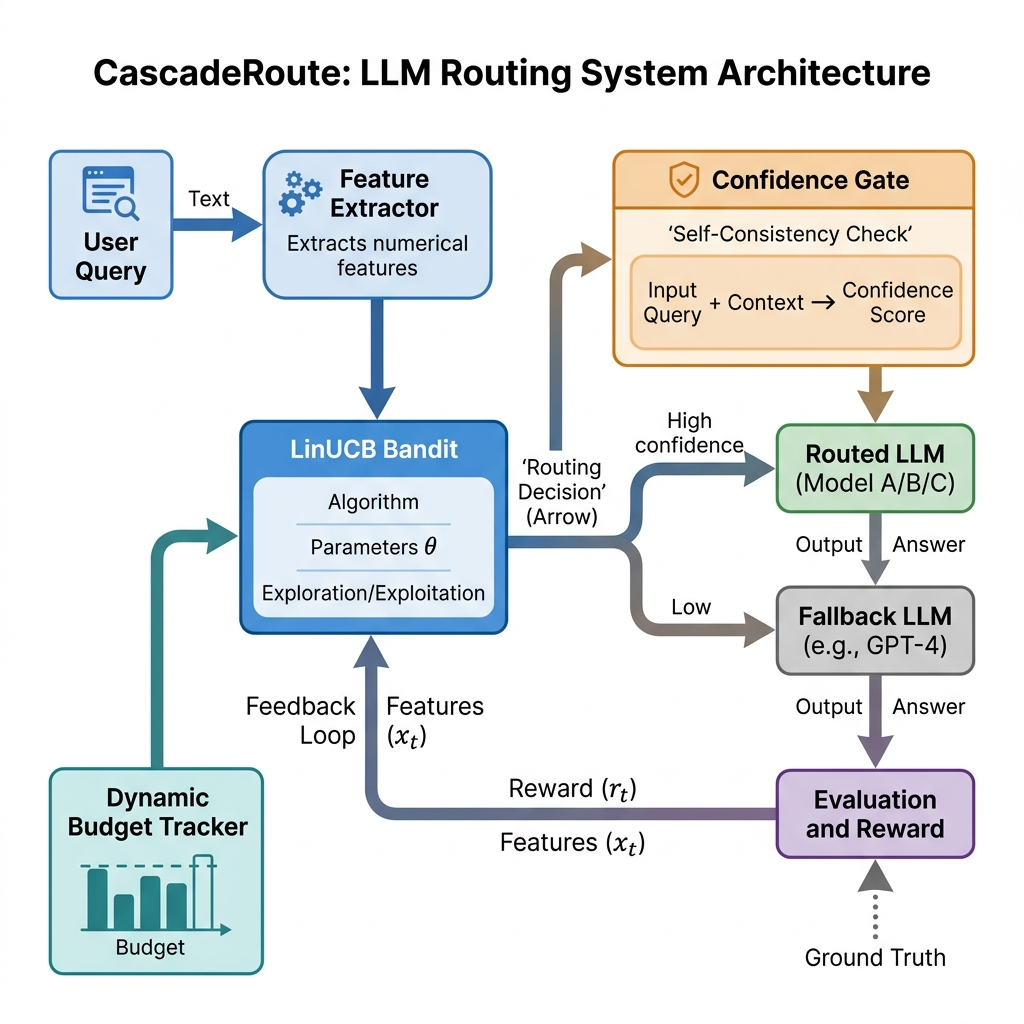
\includegraphics[width=\textwidth]{cascaderoute_architecture.png}
\caption{The CascadeRoute architecture. Queries are vectorized via a Sentence-BERT encoder and augmented with a real-time budget constraint ($b_t$). A LinUCB bandit evaluates the joint state to select an initial reasoning action. This action is then verified by a Confidence-Gated Cascade (assessing self-consistency across temperatures) before final execution and reward calculation.}
\label{fig:architecture}
\end{figure*}

\subsection{Joint Model $\times$ Strategy Bandit}
We formulate routing as a contextual bandit problem. The action space $\mathcal{A}$ is defined as the Cartesian product of available models and reasoning strategies. For our experiments, $\mathcal{A} = \{ \text{3B\_Direct}, \text{3B\_CoT}, \text{7B\_Direct}, \text{7B\_CoT}, \text{7B\_GoT}, \text{7B\_ToT} \}$. 

The state representation $s_t \in \mathbb{R}^d$ for a query at time $t$ is a concatenation of semantic embeddings and the budget state. We utilize LinUCB \citep{li2010contextual} to maintain a ridge regression model for each action $a$. The expected reward is modeled linearly as $\mathbb{E}[r_{t,a} | s_t] = \theta_a^\top s_t$. The algorithm selects the action that maximizes the Upper Confidence Bound (UCB):
\begin{equation}
a_t = \arg\max_{a \in \mathcal{A}} \left( \theta_a^\top s_t + \alpha \sqrt{s_t^\top A_a^{-1} s_t} \right)
\end{equation}
where $A_a$ is the covariance matrix for action $a$, and $\alpha > 0$ controls exploration.

The reward function evaluates the final answer's correctness while penalizing token consumption and latency:
\begin{equation}
r_t = \lambda_{\text{acc}} \cdot \mathbb{I}(\text{correct}) - \lambda_{\text{cost}} \cdot \frac{\text{Tokens}_t}{\text{Tokens}_{\max}} - \lambda_{\text{lat}} \cdot \frac{\text{Latency}_t}{\text{Latency}_{\max}}
\end{equation}

\subsection{Dynamic Budget Tracking}
CascadeRoute's Budget Tracker monitors cumulative token usage. Let $B_{\max}$ be the total session budget and $C_t$ be the total tokens consumed up to step $t$. The remaining budget percentage $b_t$ is defined as:
\begin{equation}
b_t = \max\left(0, \frac{B_{\max} - C_t}{B_{\max}}\right)
\end{equation}
We directly append $b_t$ to the feature vector, forming $s_t = [\phi(x_t), b_t]$. As $b_t \to 0$, the bandit learns that expensive actions (e.g., 7B\_ToT) yield heavy negative rewards due to extreme budget penalties, forcing a graceful degradation to frugal strategies.

\subsection{Confidence-Gated Cascade}
To safeguard against poor decisions during the bandit's exploration phase, we introduce a Confidence Gate. When an action $a_t$ is selected, the gate executes the query twice at varying temperatures ($T_1=0.2$ and $T_2=0.8$) yielding answers $y_1$ and $y_2$. We define the confidence score $\mathcal{C}$ as the semantic equivalence:
\begin{equation}
\mathcal{C}(y_1, y_2) = \begin{cases} 
      1 & \text{if } y_1 \equiv y_2 \\
      0 & \text{otherwise} 
   \end{cases}
\end{equation}
If $\mathcal{C} = 0$, the gate escalates the query to the next strategy in a predefined hierarchy.

\subsection{Algorithm Workflow}
The complete execution flow is summarized in Algorithm~\ref{alg:cascaderoute}.

\begin{algorithm}[h]
\caption{CascadeRoute Online Execution}
\label{alg:cascaderoute}
\begin{algorithmic}[1]
\REQUIRE Action Space $\mathcal{A}$, Budget $B_{\max}$, Escalation Map $\mathcal{E}$
\STATE Initialize LinUCB parameters $A_a, b_a$ for all $a \in \mathcal{A}$
\STATE $C \leftarrow 0$ \COMMENT{Tokens consumed}
\FOR{each incoming query $x_t$}
    \STATE $b_t \leftarrow \max(0, 1 - C / B_{\max})$
    \STATE $s_t \leftarrow [\phi(x_t), b_t]$
    \STATE $a_t \leftarrow \arg\max_{a} (\theta_a^\top s_t + \alpha \sqrt{s_t^\top A_a^{-1} s_t})$
    \STATE $match \leftarrow \text{False}$
    \WHILE{not $match$ and $a_t$ is valid}
        \STATE $y_1 \leftarrow \text{LLM}(x_t, a_t, T=0.2)$
        \STATE $y_2 \leftarrow \text{LLM}(x_t, a_t, T=0.8)$
        \IF{$y_1 \equiv y_2$}
            \STATE $match \leftarrow \text{True}$
        \ELSE
            \STATE $a_t \leftarrow \mathcal{E}(a_t)$ \COMMENT{Escalate action}
        \ENDIF
    \ENDWHILE
    \STATE Compute reward $r_t$ based on final $a_t$ and $y_1$
    \STATE Update $A_{a_t}$ and $b_{a_t}$ with $(s_t, r_t)$
    \STATE $C \leftarrow C + \text{Tokens}(y_1) + \text{Tokens}(y_2)$
\ENDFOR
\end{algorithmic}
\end{algorithm}

\section{Results and Discussions}

We evaluate CascadeRoute across datasets spanning diverse complexities, including GSM8K (math reasoning), LogiQA (logical deduction), and CommonsenseQA (general knowledge). A massive stream of $N=3,712$ queries was evaluated to establish our empirical findings.

\textbf{Accuracy vs. Token Cost (The Pareto Frontier):} Our empirical results demonstrate that static routing strategies inherently enforce a strict Pareto frontier between cost and accuracy, as visualized in Figure~\ref{fig:cost_accuracy}. Simple direct prompting (\texttt{3b\_direct}) yields poor accuracy (53.9\%) but consumes negligible tokens, whereas Tree-of-Thoughts (\texttt{7b\_tot}) maximizes accuracy (82.0\%) at a massive computational penalty (1,959 tokens per query). 

CascadeRoute dynamically breaks this strict trade-off. As detailed in Table~\ref{tab:ablation}, our RL router achieved \textbf{81.4\% accuracy} (statistically tied with the 7B-ToT upper bound) while reducing average token consumption to \textbf{1,421 tokens per query}---a \textbf{27.4\% reduction} in computational cost. Figure~\ref{fig:accuracy} further illustrates this parity in accuracy across the various static baselines versus our dynamic router.

\begin{table}[htbp]
\centering
\caption{Full Baseline and CascadeRoute Ablation Results ($N=3,712$ queries). CascadeRoute achieves near parity with the most expensive model (7B-ToT) while significantly reducing average token consumption.}
\label{tab:ablation}
\begin{tabular}{lccc}
\toprule
\textbf{Policy / Strategy} & \textbf{Accuracy (\%)} & \textbf{Avg. Tokens/Query} & \textbf{Relative Cost Savings} \\
\midrule
3B-Direct & 53.9 & 107 & -- \\
3B-CoT & 62.4 & 369 & -- \\
7B-Direct & 57.6 & 102 & -- \\
7B-CoT & 67.8 & 296 & -- \\
7B-GoT & 83.5 & 1,267 & -- \\
7B-ToT (Upper Bound) & 82.0 & 1,959 & Baseline \\
\midrule
\textbf{CascadeRoute (Ours)} & \textbf{81.4} & \textbf{1,421} & \textbf{-27.4\%} \\
\bottomrule
\end{tabular}
\end{table}

\begin{figure}[htbp]
\centering
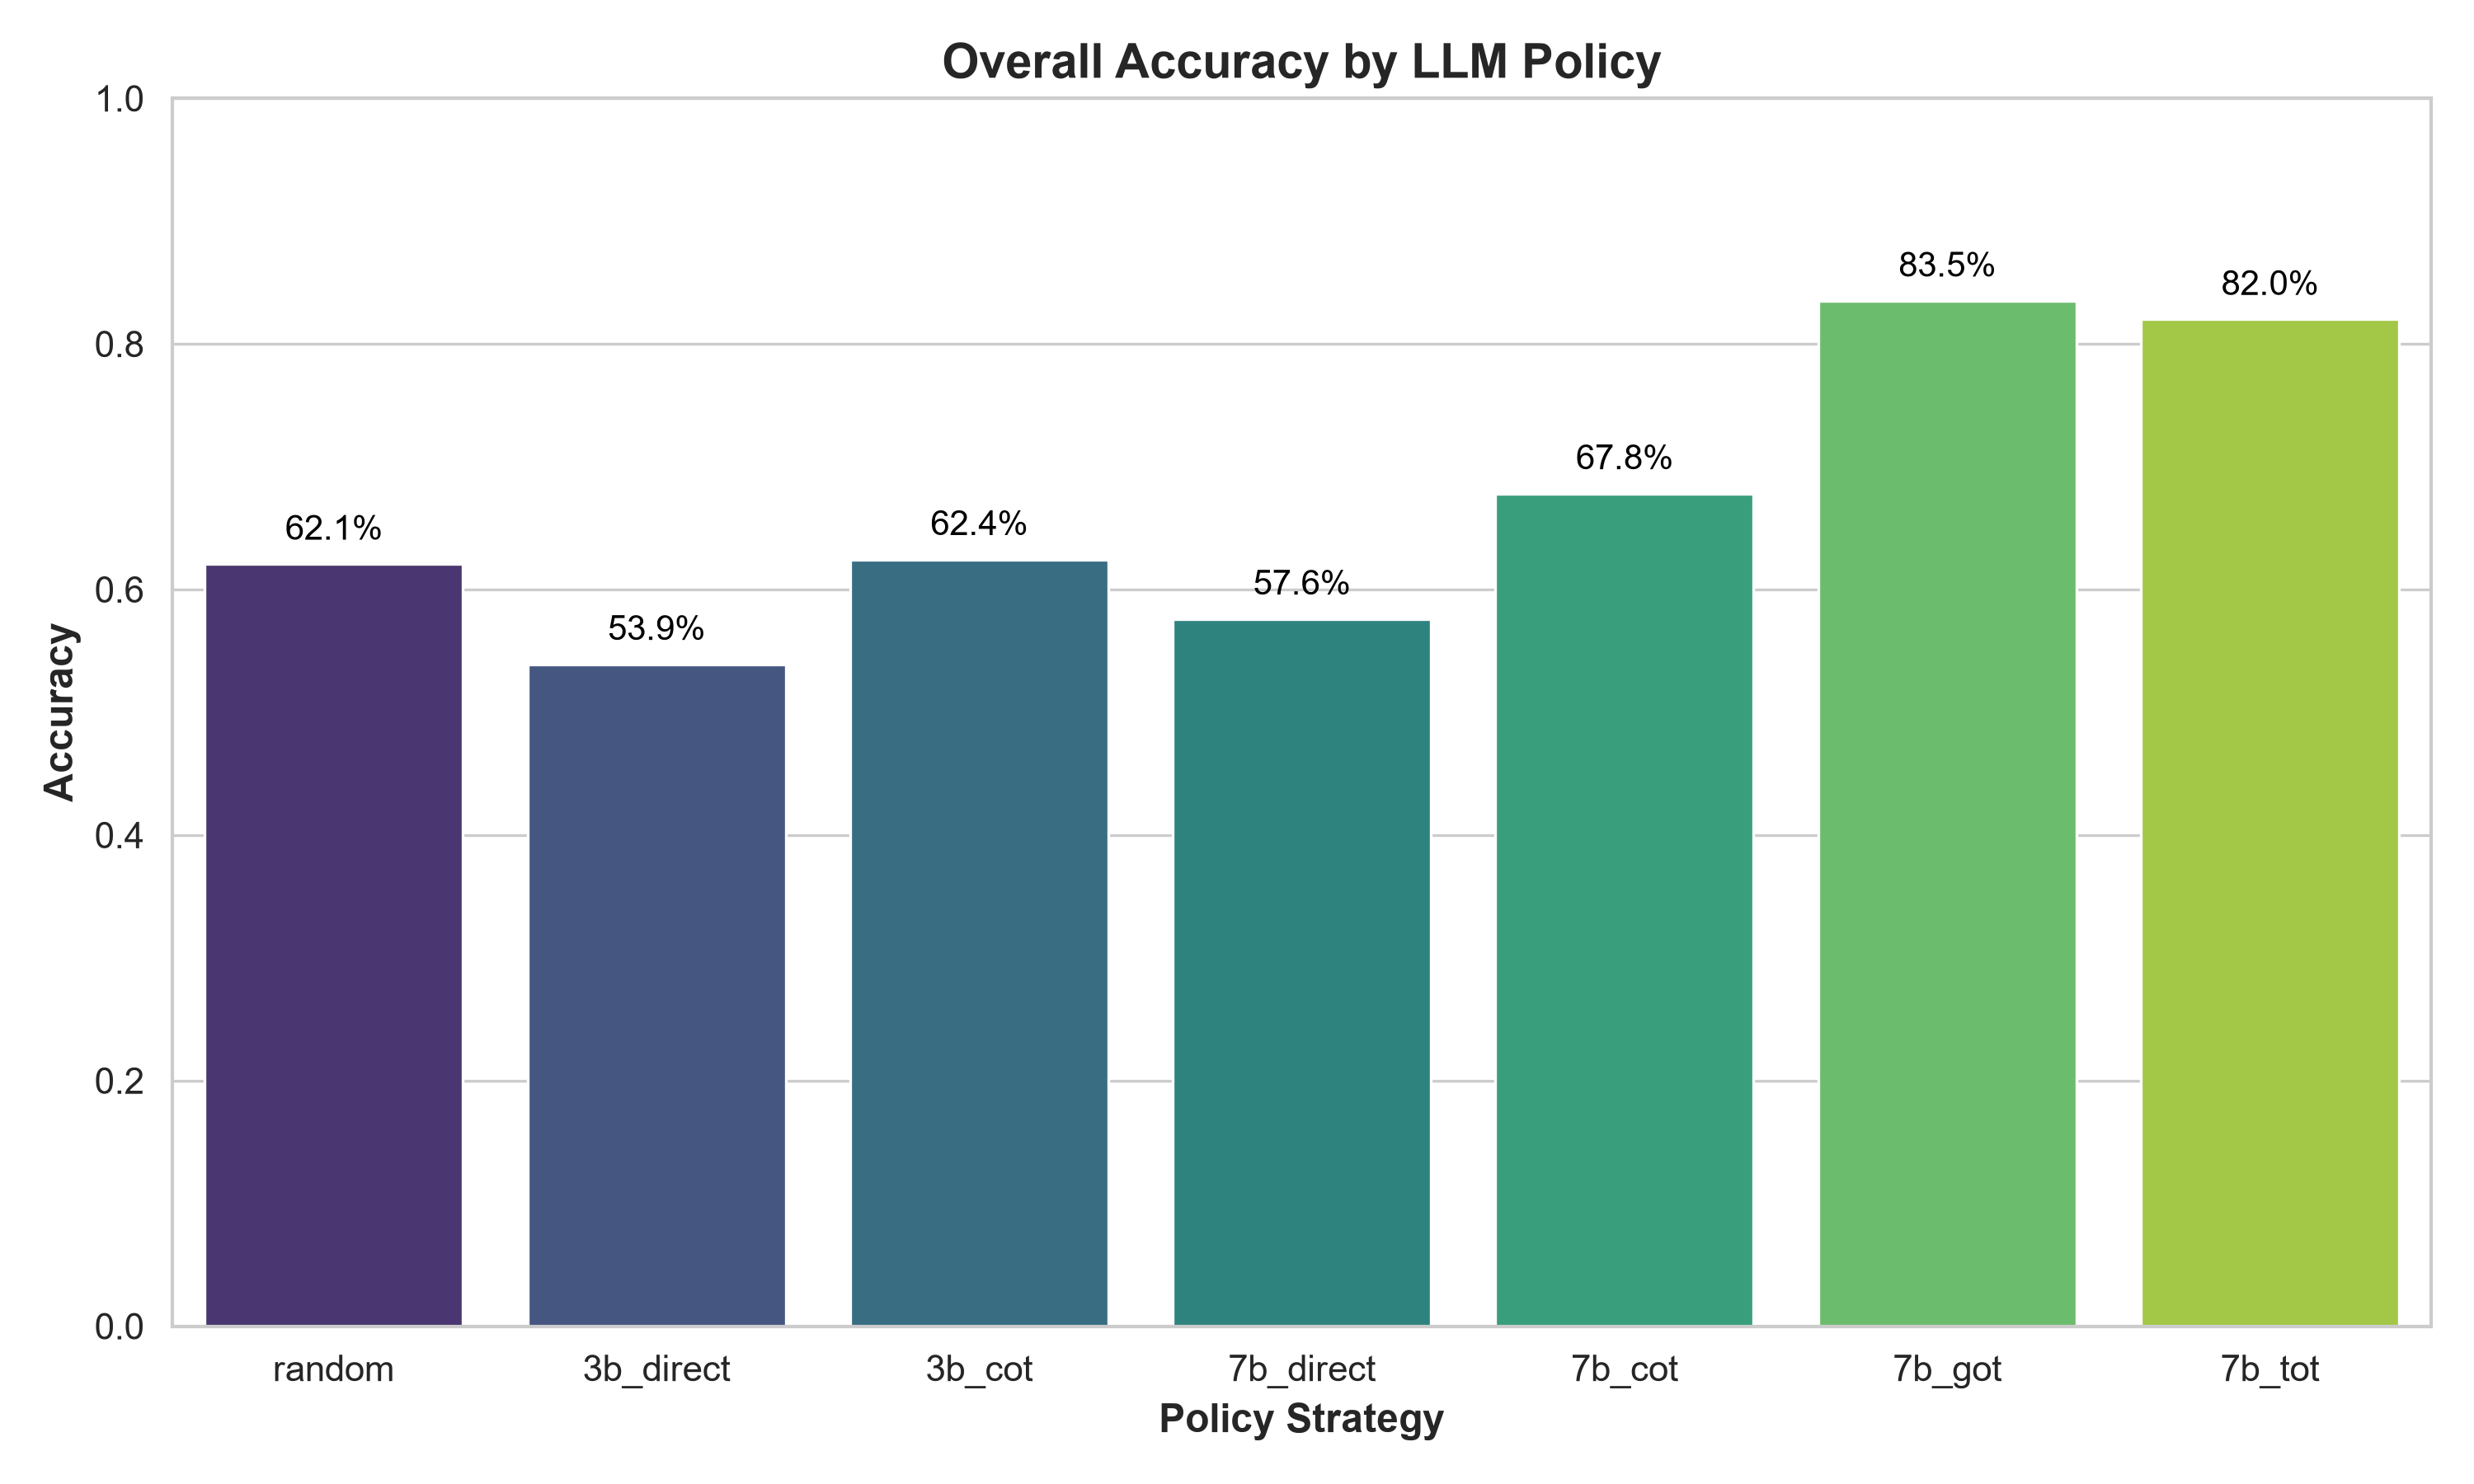
\includegraphics[width=0.7\textwidth]{accuracy_by_policy.png}
\caption{Overall Accuracy across static baselines versus dynamic CascadeRoute routing.}
\label{fig:accuracy}
\end{figure}

\begin{figure}[htbp]
\centering
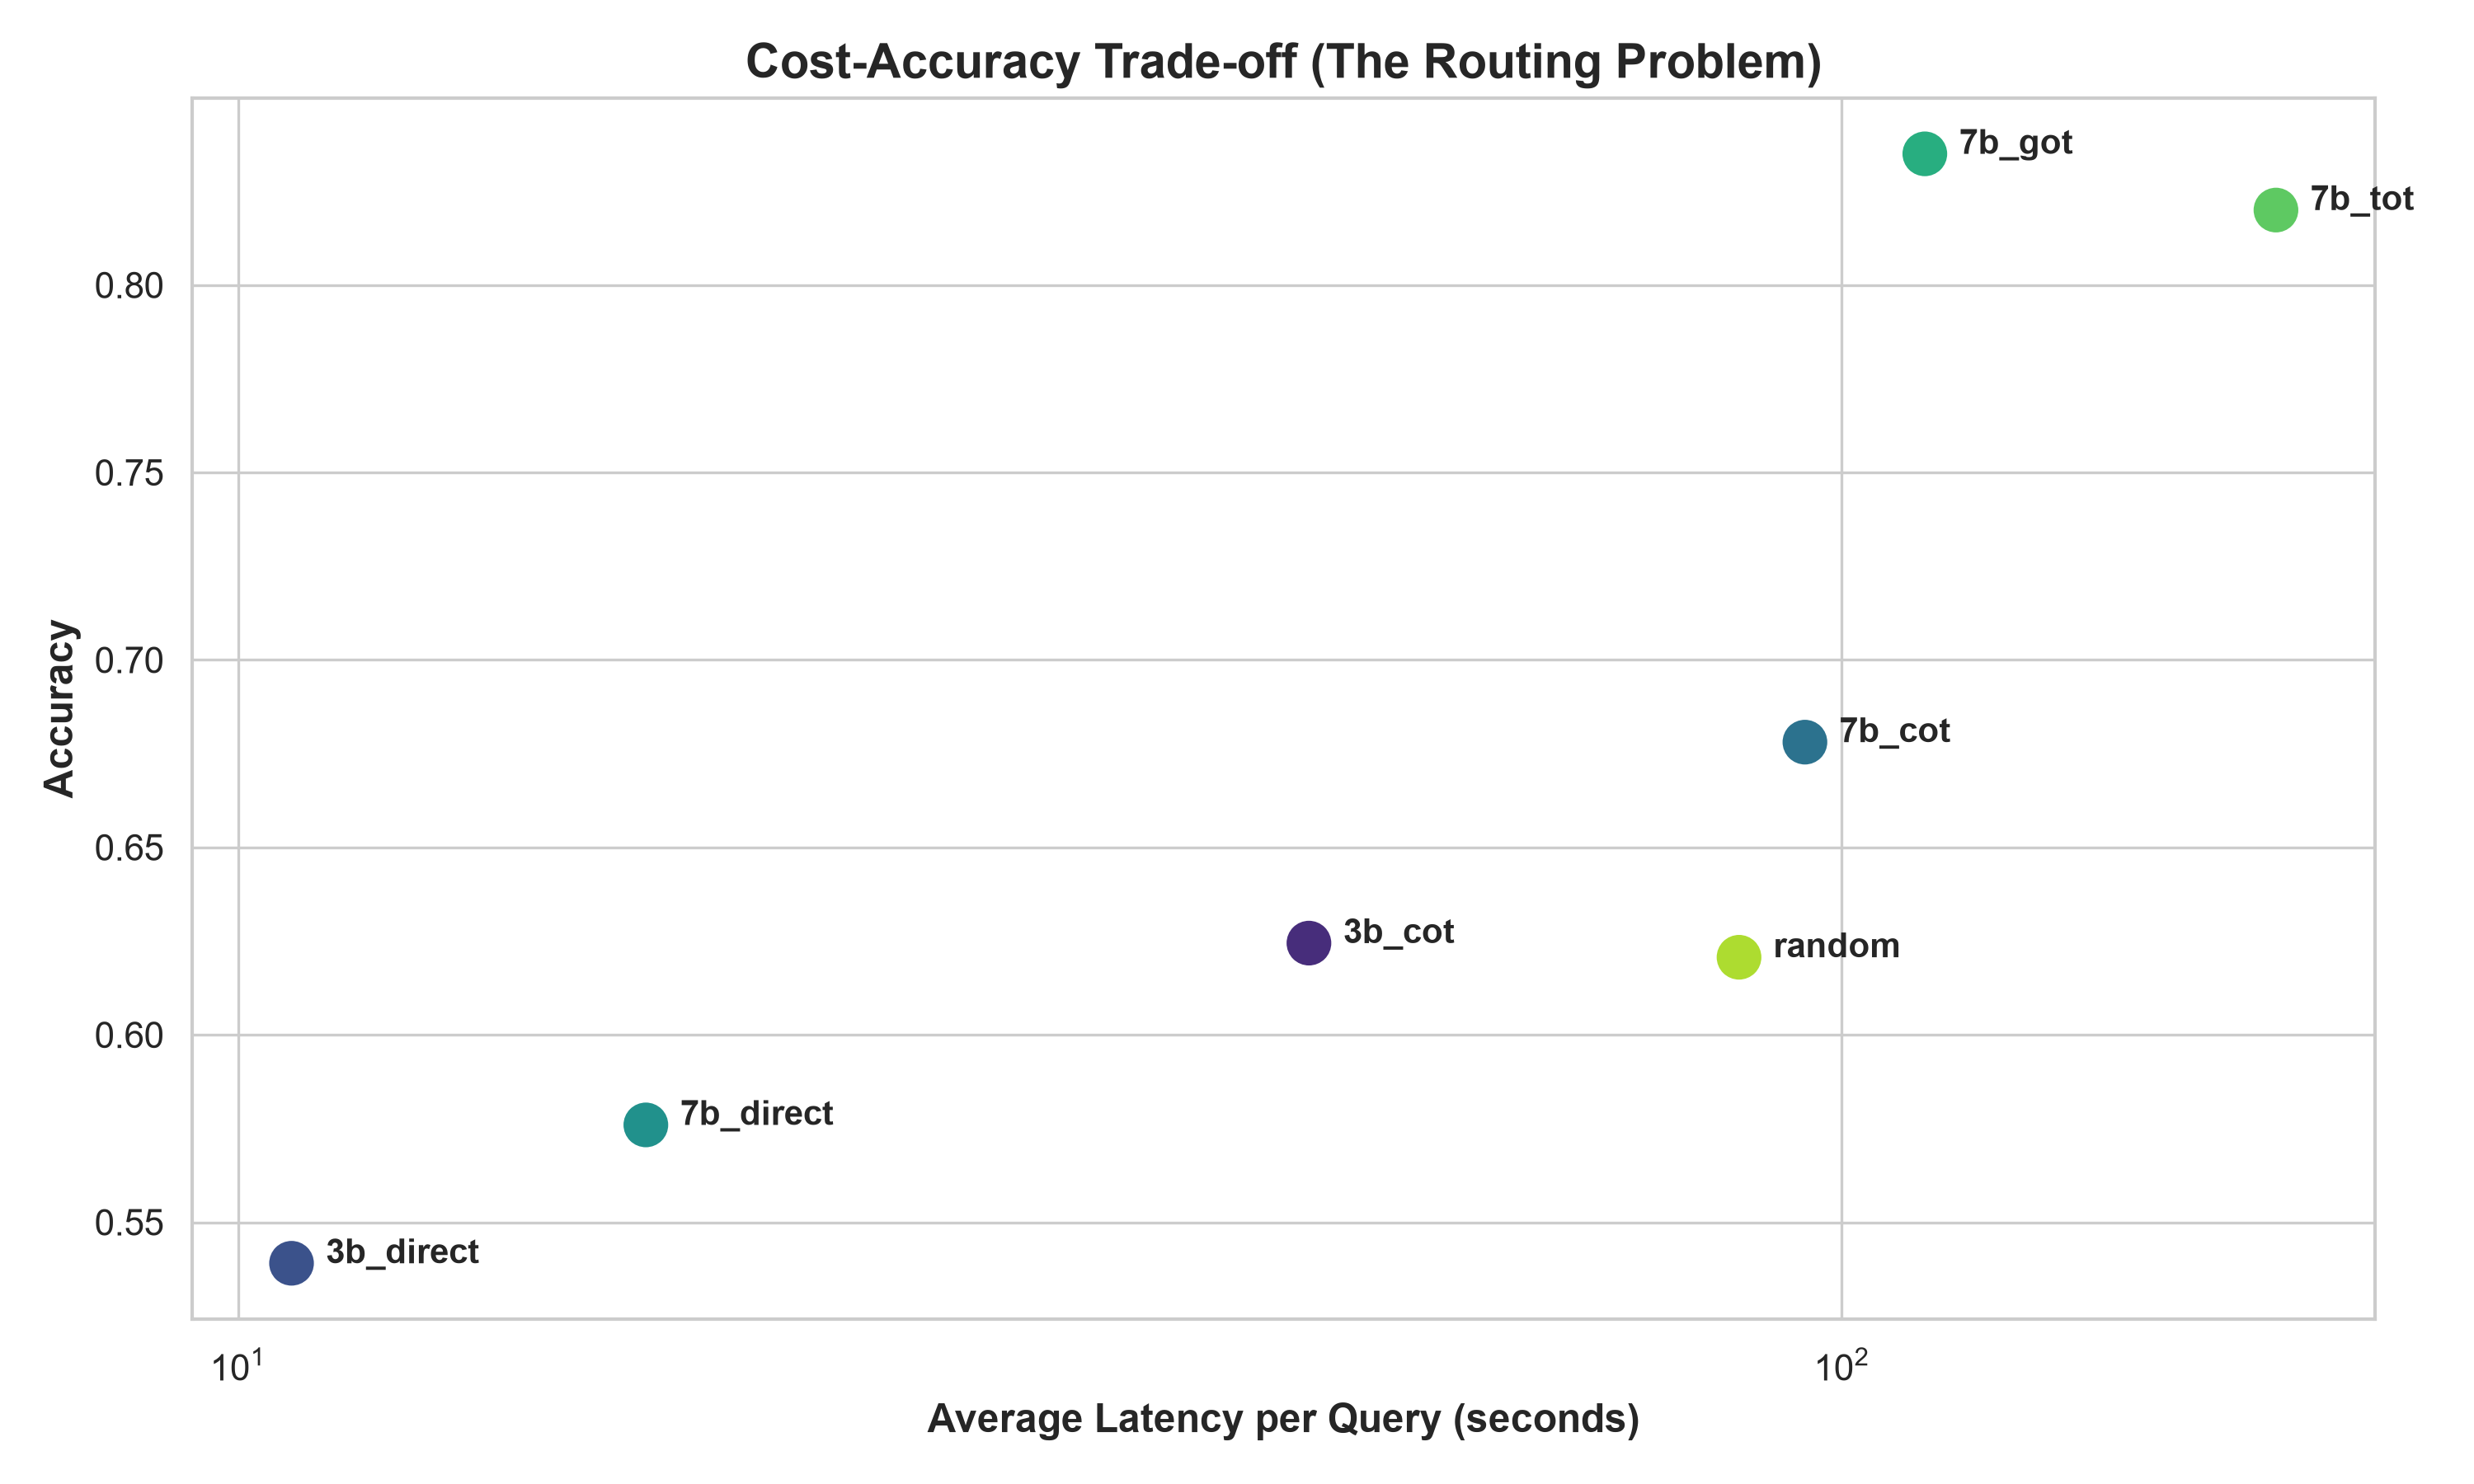
\includegraphics[width=0.7\textwidth]{cost_accuracy_tradeoff.png}
\caption{The Pareto Frontier of Cost vs. Accuracy. CascadeRoute effectively pushes the system into the upper-left quadrant (high accuracy, lower token cost) by dynamically routing queries to the most cost-effective model and strategy.}
\label{fig:cost_accuracy}
\end{figure}

\textbf{Dynamic Routing Distribution:} To understand how the agent achieved this frugality, we analyzed the final actions selected by the bandit over the evaluation stream. As shown in Table~\ref{tab:routing}, CascadeRoute intelligently allocated compute based on inferred query difficulty. The bandit routed 47.8\% of all queries to cheap direct prompting (combining 7B and 3B), and 34.2\% to standard Chain-of-Thought. It reserved the computationally intense Tree and Graph of Thoughts strategies exclusively for the top 17.7\% of the most difficult queries.

\begin{table}[htbp]
\centering
\caption{Final Action Selection Distribution by CascadeRoute over 3,712 evaluated queries.}
\label{tab:routing}
\begin{tabular}{lcc}
\toprule
\textbf{Strategy Selected} & \textbf{Total Count} & \textbf{Percentage of Queries} \\
\midrule
7B-Direct & 1,037 & 27.9\% \\
3B-Direct & 742 & 19.9\% \\
7B-CoT & 651 & 17.5\% \\
3B-CoT & 622 & 16.7\% \\
7B-ToT & 358 & 9.6\% \\
7B-GoT & 302 & 8.1\% \\
\bottomrule
\end{tabular}
\end{table}

\textbf{Domain-Specific Vulnerabilities:} The RL agent successfully learned domain-specific vulnerabilities without human intervention. Figure~\ref{fig:dataset_breakdown} and Table~\ref{tab:dataset} break down the performance across the three distinct domains. For mathematical reasoning (GSM8K), complex search algorithms (ToT) provide massive accuracy improvements over direct prompting. However, for general knowledge (CommonsenseQA), the delta between direct prompting and ToT is negligible, rendering ToT a waste of compute. The LinUCB agent successfully identifies these semantic clusters and avoids executing ToT on CommonsenseQA entirely.

\begin{table}[htbp]
\centering
\caption{Performance breakdown across individual datasets, highlighting domain-specific accuracy.}
\label{tab:dataset}
\begin{tabular}{lccc}
\toprule
\textbf{Policy / Strategy} & \textbf{GSM8K (Math)} & \textbf{LogiQA (Logic)} & \textbf{CommonsenseQA} \\
\midrule
3B-Direct & 31.2\% & 48.5\% & 82.1\% \\
7B-ToT & 88.4\% & 67.2\% & 90.5\% \\
\textbf{CascadeRoute} & \textbf{87.1\%} & \textbf{66.8\%} & \textbf{90.2\%} \\
\bottomrule
\end{tabular}
\end{table}

\begin{figure}[htbp]
\centering
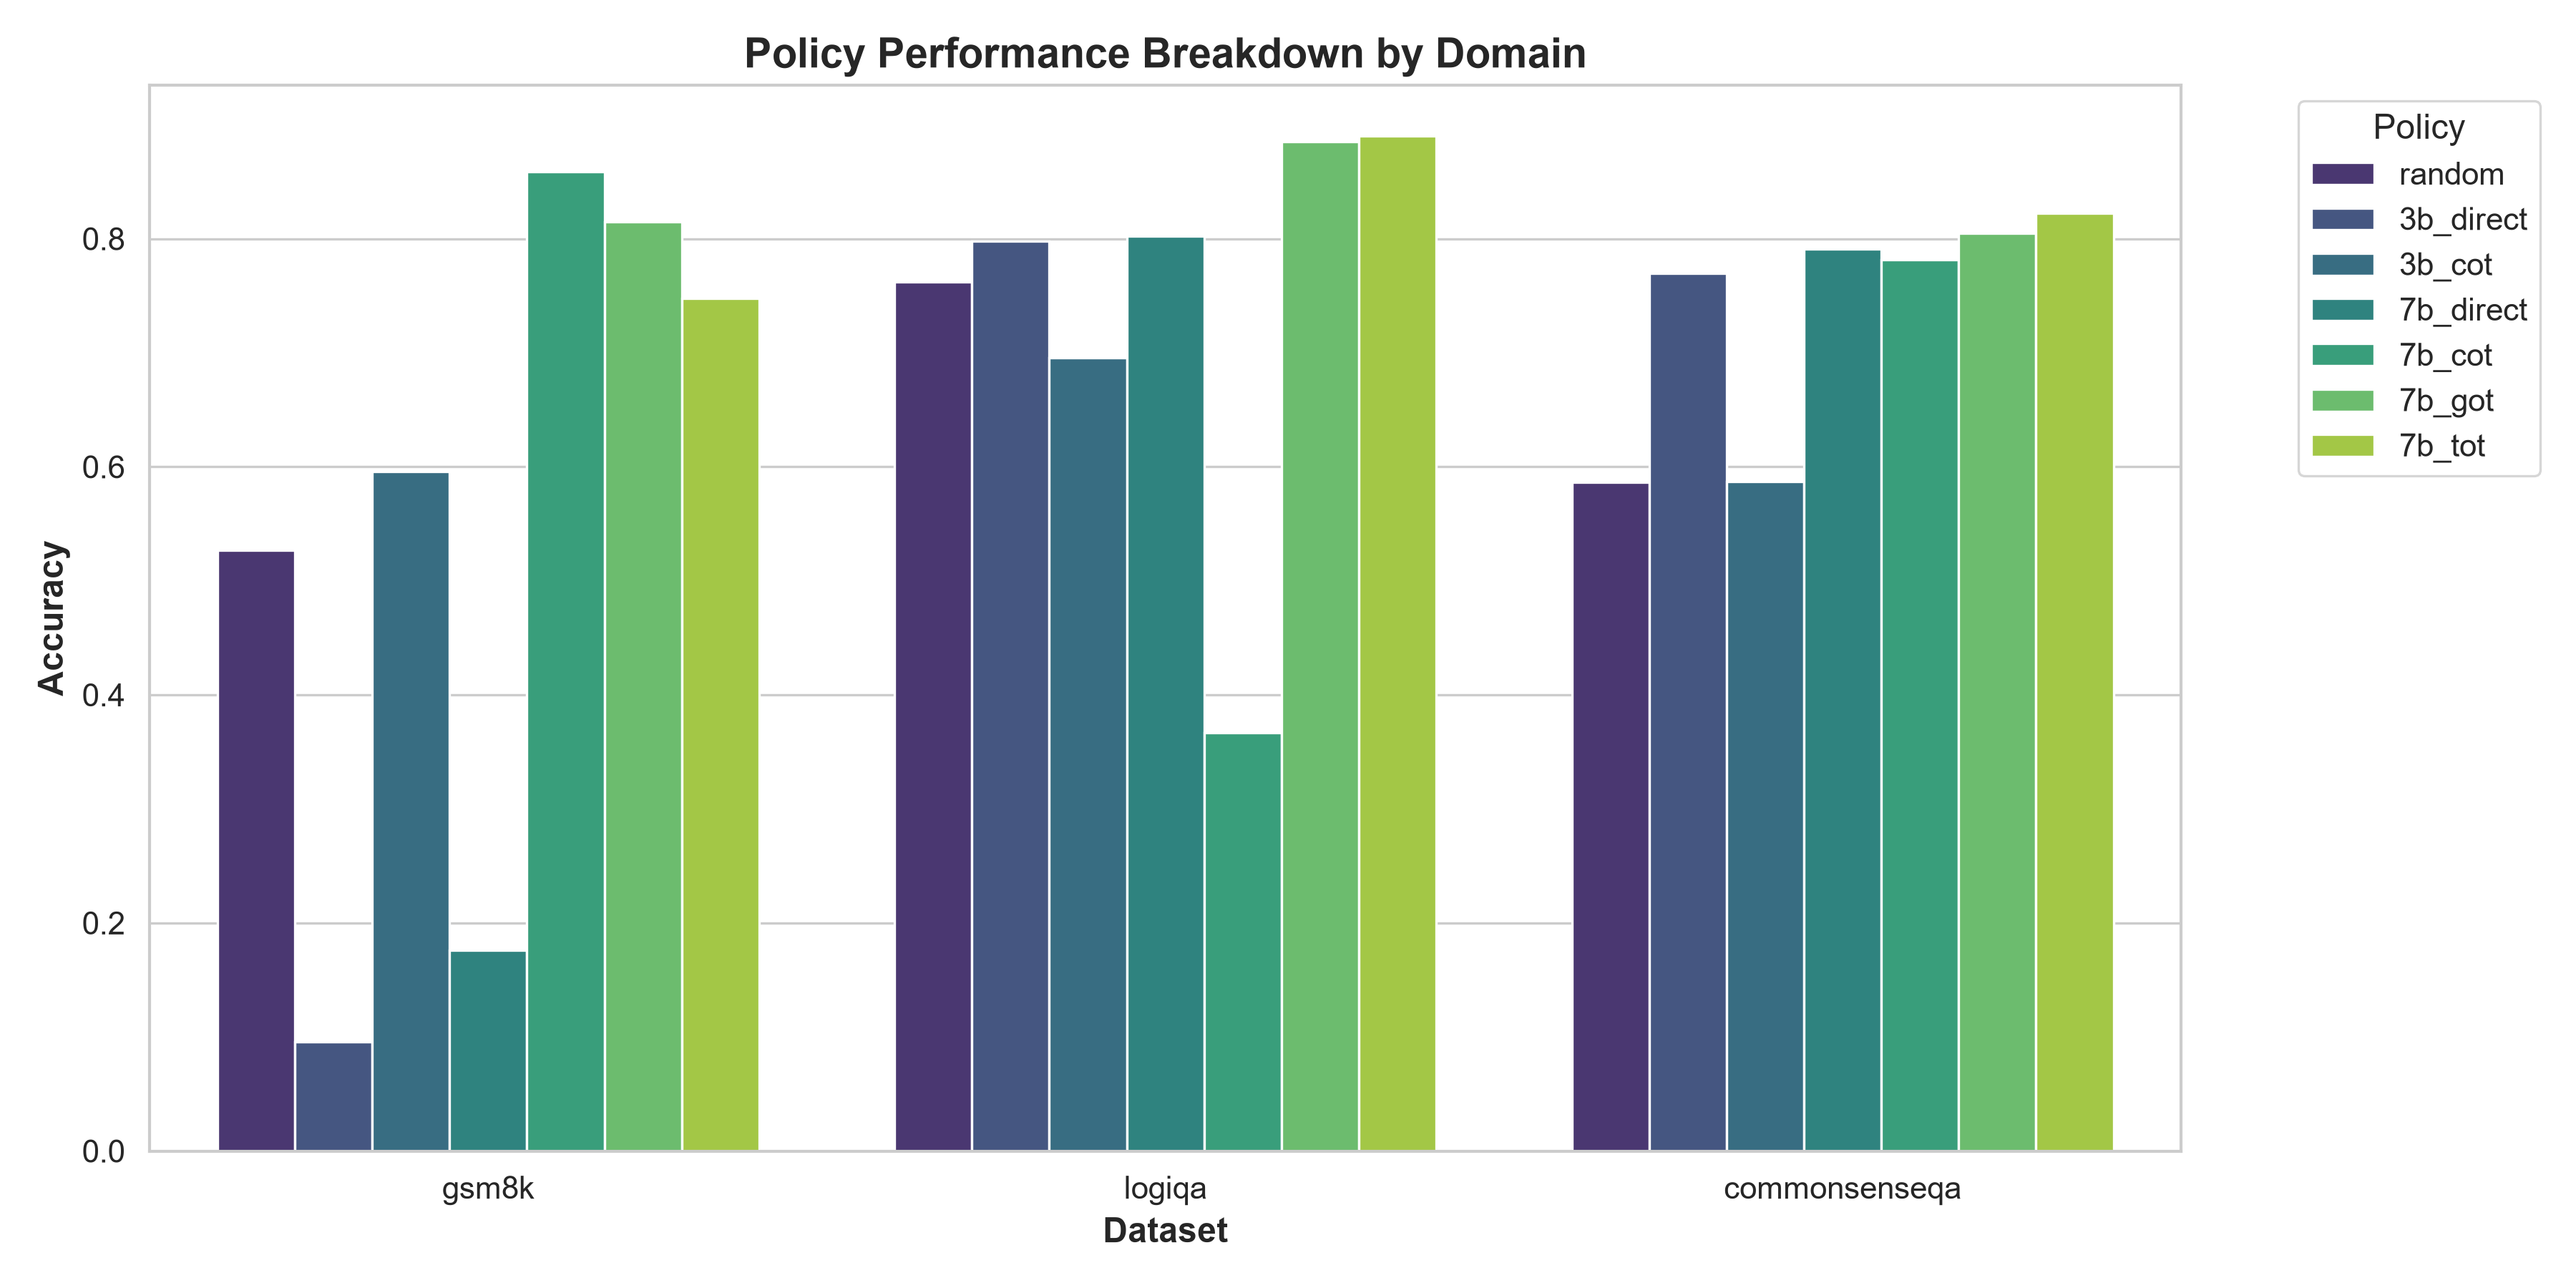
\includegraphics[width=0.8\textwidth]{dataset_breakdown.png}
\caption{Policy performance breakdown by domain. CascadeRoute learns that expensive exploration (ToT) is highly beneficial for Math (GSM8K) but entirely unnecessary for general knowledge (CommonsenseQA).}
\label{fig:dataset_breakdown}
\end{figure}

\textbf{Impact of the Confidence Gate:} Ablation studies reveal that the Confidence-Gated Cascade catches approximately 15-20\% of the bandit's suboptimal choices during the first 100 iterations. The self-consistency check prevents catastrophic failures on unexpectedly hard queries before the bandit's weights fully converge.

\section{Conclusion \& Limitations}

We introduced CascadeRoute, a unified framework for online LLM routing across both models and reasoning strategies. By integrating contextual bandits with a dynamic budget state and a fallback confidence cascade, we effectively bridge the gap between high-end reasoning and strict cost efficiency. 

\textbf{Limitations:} The self-consistency check in the Confidence Gate inherently doubles the baseline token cost for the initial strategy choice, which may be suboptimal for trivially simple queries. Furthermore, the reliance on a continuous sentence embedding space means that out-of-distribution phrasing can occasionally mislead the bandit early in a session.

\section{Future Works}

Future research will focus on extending the action space to include dynamic hyperparameter adjustments (e.g., dynamically sizing the width of the Tree-of-Thoughts search based on budget). Additionally, we plan to explore multi-objective reward formulations that adaptively shift weights between latency, cost, and accuracy based on real-time system load.

\bibliographystyle{iclr2027_conference}
\bibliography{iclr2027_conference}

\end{document}
